\section{Linear Algebra}

% show diagrams with terms, then show squaring
\frame{
    \frametitle{3D Coupling Dependence}
    \begin{figure}
    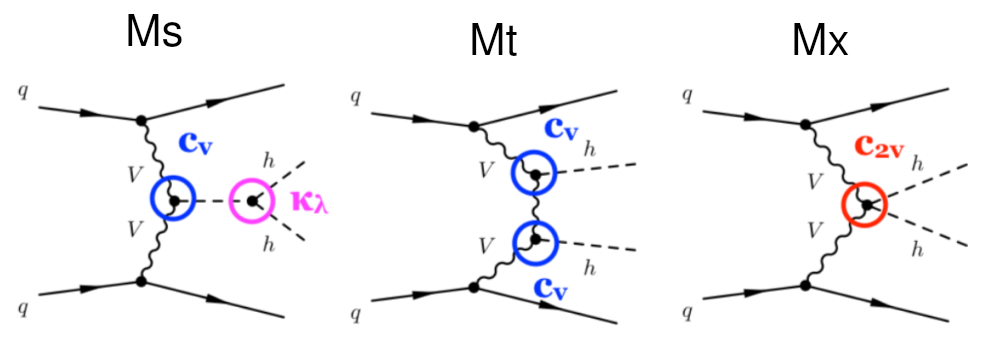
\includegraphics[width=0.6\linewidth,height=0.6\textheight,keepaspectratio]{vbf-hh_diagrams2b}
    \end{figure}
    $ \sigma = | \kv \kl M_s + \kv^2 M_t + \kvv M_x |^2 = $

    \vspace{10mm}

    $ \kv^2 \kl^2 M_s^2 + \kv^4 M_t^2 + \kvv^2 M_x^2 
    + \kv^3 \kl (M_s^* M_t + M_t^* M_s) 
    + \kv \kl \kvv (M_s^* M_x + M_x^* M_s ) 
    + \kv^2 \kvv (M_t^* M_x + M_x^* M_t )$

    \vspace{10mm}

    $ \sigma = \kv^2 \kl^2 a_1 + \kv^4 a_2 + \kvv^2 a_3 + \kv^3 \kl a_4 + \kv \kl \kvv a_5 + \kv^2 \kvv a_6 $
}

% 6 variables, six equations, make a mess
\frame{
    \frametitle{6 Unknowns: Solve With 6 Equations}

    \vspace{5mm}

    \foreach \index in {1,2,3,4,5,6}{
        { \small $ \sigma_\index = \fkv{\index}^2 \fkl{\index}^2 a_1 + \fkv{\index}^4 a_2 + \fkvv{\index}^2 a_3 + \fkv{\index}^3 \fkl{\index} a_4 + \fkv{\index} \fkl{\index} \fkvv{\index} a_5 + \fkv{\index}^2 \fkvv{\index} a_6 $ }

        \vspace{5mm}
    }
}

% convert to matrix, show nice matrix solution
\frame{
    \frametitle{Linear Algebra Makes this Simple}

    \begin{columns}[T]
        \begin{column}{0.18\textwidth}
            $ \vec{\sigma} = \begin{pmatrix} \sigma_1 \\ \sigma_2 \\ \sigma_3 \\ \sigma_4 \\ \sigma_5 \\ \sigma_6 \end{pmatrix} $
        \end{column}
        \begin{column}{0.15\textwidth}
            $ \vec{a} = \begin{pmatrix} a_1 \\ a_2 \\ a_3 \\ a_4 \\ a_5 \\ a_6 \end{pmatrix} $
        \end{column}
        \begin{column}{0.25\textwidth}
            $ \vec{f} = \begin{pmatrix} \kv^2 \kl^2 \\ \kv^4 \\ \kvv^2 \\ \kv^3 \kl \\ \kv \kl \kvv \\ \kv^2 \kvv \end{pmatrix} $
        \end{column}
        \begin{column}{0.4\textwidth}
            $ F = \begin{pmatrix}
                \vec{f}(\fkvv{1}, \fkl{1}, \fkv{1}) \\
                \vec{f}(\fkvv{2}, \fkl{2}, \fkv{2}) \\
                \vec{f}(\fkvv{3}, \fkl{3}, \fkv{3}) \\
                \vec{f}(\fkvv{4}, \fkl{4}, \fkv{4}) \\
                \vec{f}(\fkvv{5}, \fkl{5}, \fkv{5}) \\
                \vec{f}(\fkvv{6}, \fkl{6}, \fkv{6}) \\
            \end{pmatrix} $
        \end{column}
    \end{columns}

    \vspace{10mm}

    $ \vec{\sigma} = F \bullet \vec{a} \; \Longrightarrow \; \vec{a} = F^{-1} \bullet \vec{\sigma} $

    \vspace{10mm}

    $ \boxed{ \sigma(\kvv,\kl,\kv) = \vec{f}(\kvv,\kl,\kv) \bullet F^{-1} \bullet \vec{\sigma} } $
}
